\documentclass[preprint, 3p,
authoryear]{elsarticle} %review=doublespace preprint=single 5p=2 column
%%% Begin My package additions %%%%%%%%%%%%%%%%%%%

\usepackage[hyphens]{url}

  \journal{Environmental Modelling \& Software} % Sets Journal name

\usepackage{graphicx}
%%%%%%%%%%%%%%%% end my additions to header

\usepackage[T1]{fontenc}
\usepackage{lmodern}
\usepackage{amssymb,amsmath}
% TODO: Currently lineno needs to be loaded after amsmath because of conflict
% https://github.com/latex-lineno/lineno/issues/5
\usepackage{lineno} % add
  \linenumbers % turns line numbering on
\usepackage{ifxetex,ifluatex}
\usepackage{fixltx2e} % provides \textsubscript
% use upquote if available, for straight quotes in verbatim environments
\IfFileExists{upquote.sty}{\usepackage{upquote}}{}
\ifnum 0\ifxetex 1\fi\ifluatex 1\fi=0 % if pdftex
  \usepackage[utf8]{inputenc}
\else % if luatex or xelatex
  \usepackage{fontspec}
  \ifxetex
    \usepackage{xltxtra,xunicode}
  \fi
  \defaultfontfeatures{Mapping=tex-text,Scale=MatchLowercase}
  \newcommand{\euro}{€}
\fi
% use microtype if available
\IfFileExists{microtype.sty}{\usepackage{microtype}}{}
\usepackage[]{natbib}
\bibliographystyle{plainnat}

\usepackage{graphicx}
\ifxetex
  \usepackage[setpagesize=false, % page size defined by xetex
              unicode=false, % unicode breaks when used with xetex
              xetex]{hyperref}
\else
  \usepackage[unicode=true]{hyperref}
\fi
\hypersetup{breaklinks=true,
            bookmarks=true,
            pdfauthor={},
            pdftitle={robspack An R package for processing atmospheric greenhouse gas observations in NOAA's ObsPack},
            colorlinks=false,
            urlcolor=blue,
            linkcolor=magenta,
            pdfborder={0 0 0}}

\setcounter{secnumdepth}{5}
% Pandoc toggle for numbering sections (defaults to be off)

% Pandoc syntax highlighting
\usepackage{color}
\usepackage{fancyvrb}
\newcommand{\VerbBar}{|}
\newcommand{\VERB}{\Verb[commandchars=\\\{\}]}
\DefineVerbatimEnvironment{Highlighting}{Verbatim}{commandchars=\\\{\}}
% Add ',fontsize=\small' for more characters per line
\usepackage{framed}
\definecolor{shadecolor}{RGB}{248,248,248}
\newenvironment{Shaded}{\begin{snugshade}}{\end{snugshade}}
\newcommand{\AlertTok}[1]{\textcolor[rgb]{0.94,0.16,0.16}{#1}}
\newcommand{\AnnotationTok}[1]{\textcolor[rgb]{0.56,0.35,0.01}{\textbf{\textit{#1}}}}
\newcommand{\AttributeTok}[1]{\textcolor[rgb]{0.13,0.29,0.53}{#1}}
\newcommand{\BaseNTok}[1]{\textcolor[rgb]{0.00,0.00,0.81}{#1}}
\newcommand{\BuiltInTok}[1]{#1}
\newcommand{\CharTok}[1]{\textcolor[rgb]{0.31,0.60,0.02}{#1}}
\newcommand{\CommentTok}[1]{\textcolor[rgb]{0.56,0.35,0.01}{\textit{#1}}}
\newcommand{\CommentVarTok}[1]{\textcolor[rgb]{0.56,0.35,0.01}{\textbf{\textit{#1}}}}
\newcommand{\ConstantTok}[1]{\textcolor[rgb]{0.56,0.35,0.01}{#1}}
\newcommand{\ControlFlowTok}[1]{\textcolor[rgb]{0.13,0.29,0.53}{\textbf{#1}}}
\newcommand{\DataTypeTok}[1]{\textcolor[rgb]{0.13,0.29,0.53}{#1}}
\newcommand{\DecValTok}[1]{\textcolor[rgb]{0.00,0.00,0.81}{#1}}
\newcommand{\DocumentationTok}[1]{\textcolor[rgb]{0.56,0.35,0.01}{\textbf{\textit{#1}}}}
\newcommand{\ErrorTok}[1]{\textcolor[rgb]{0.64,0.00,0.00}{\textbf{#1}}}
\newcommand{\ExtensionTok}[1]{#1}
\newcommand{\FloatTok}[1]{\textcolor[rgb]{0.00,0.00,0.81}{#1}}
\newcommand{\FunctionTok}[1]{\textcolor[rgb]{0.13,0.29,0.53}{\textbf{#1}}}
\newcommand{\ImportTok}[1]{#1}
\newcommand{\InformationTok}[1]{\textcolor[rgb]{0.56,0.35,0.01}{\textbf{\textit{#1}}}}
\newcommand{\KeywordTok}[1]{\textcolor[rgb]{0.13,0.29,0.53}{\textbf{#1}}}
\newcommand{\NormalTok}[1]{#1}
\newcommand{\OperatorTok}[1]{\textcolor[rgb]{0.81,0.36,0.00}{\textbf{#1}}}
\newcommand{\OtherTok}[1]{\textcolor[rgb]{0.56,0.35,0.01}{#1}}
\newcommand{\PreprocessorTok}[1]{\textcolor[rgb]{0.56,0.35,0.01}{\textit{#1}}}
\newcommand{\RegionMarkerTok}[1]{#1}
\newcommand{\SpecialCharTok}[1]{\textcolor[rgb]{0.81,0.36,0.00}{\textbf{#1}}}
\newcommand{\SpecialStringTok}[1]{\textcolor[rgb]{0.31,0.60,0.02}{#1}}
\newcommand{\StringTok}[1]{\textcolor[rgb]{0.31,0.60,0.02}{#1}}
\newcommand{\VariableTok}[1]{\textcolor[rgb]{0.00,0.00,0.00}{#1}}
\newcommand{\VerbatimStringTok}[1]{\textcolor[rgb]{0.31,0.60,0.02}{#1}}
\newcommand{\WarningTok}[1]{\textcolor[rgb]{0.56,0.35,0.01}{\textbf{\textit{#1}}}}

% tightlist command for lists without linebreak
\providecommand{\tightlist}{%
  \setlength{\itemsep}{0pt}\setlength{\parskip}{0pt}}

% From pandoc table feature
\usepackage{longtable,booktabs,array}
\usepackage{calc} % for calculating minipage widths
% Correct order of tables after \paragraph or \subparagraph
\usepackage{etoolbox}
\makeatletter
\patchcmd\longtable{\par}{\if@noskipsec\mbox{}\fi\par}{}{}
\makeatother
% Allow footnotes in longtable head/foot
\IfFileExists{footnotehyper.sty}{\usepackage{footnotehyper}}{\usepackage{footnote}}
\makesavenoteenv{longtable}






\begin{document}


\begin{frontmatter}

  \title{robspack An R package for processing atmospheric greenhouse gas
observations in NOAA's ObsPack}
    \author[a,b]{Sergio Ibarra-Espinosa%
  \corref{cor1}%
  \fnref{1}}
   \ead{sergio.ibarra-espinosa@noaa.gov} 
    \author[b]{Lei Hu%
  %
  }
   \ead{lhu@noaa.gov} 
      \affiliation[a]{
    organization={Cooperative Institute for Research in Environmental
Sciences, CU Boulder},addressline={216 UCB, University of Colorado
Boulder
campus},city={Boulder},postcode={80309},state={Colorado},country={United
States},}
    \affiliation[b]{
    organization={NOAA Global Monitoring Laboratory},addressline={325
Broadway},postcode={80309},state={Colorado},country={United States},}
    \cortext[cor1]{Corresponding author}
    \fntext[1]{This is the first author footnote.}
  
  \begin{abstract}
  In this study, we present a new open-source R package
  \texttt{robspack}, to read, process, select, and plot NOAA Observation
  Package (ObsPack) data products. We use a methane ObsPack data product
  as an example in this code base, but it can be easily modified to
  analyze ObsPack products for other greenhouse gasses. The R package
  starts with creating a catalog of all ObsPack files in each product.
  It then reads all files and creates one database. While reading each
  ObsPack file, it extracts site elevation and time zone information
  from the file header and calculates sampling altitude in meters above
  ground level and local time for individual samping events. Finally, it
  processes and selects observations for inverse modeling purposes. This
  package imports functions from data.table R package, which contains C
  bindings with parallel implementation via Open-MP \citep{dt}.
  data.table is faster than other Python, Julia and R implementations
  for data-science, providing a strong basis for robspack. robspack
  provides functions to perform these tasks in a transparent and
  efficient way, supporting open-source communities in environmental
  sciences.
  \end{abstract}
    \begin{keyword}
    ObsPack \sep NOAA \sep 
    Greenhouse gases
  \end{keyword}
  
 \end{frontmatter}

\hypertarget{introduction}{%
\section{Introduction}\label{introduction}}

The world is experiencing an accelerated global warming due to the
accumulation of greenhouse gases (GHG) since the industrial revolution
\citep{us2018}. Greenhouse gas observations are critical to monitor the
state of the atmosphere, quantify present and historical emissions, and
understand global climate change. During the 21th Conference of Parties
(COP21), it was established the Paris Accord, a multilateral effort
reduce greenhouse emissions in order to limit the temperature increment
of 1.5 degrees \citep{rhodes20162015}. Methane is a greenhouse gas
responsible for half of the temperature increase since preindustrial
levels. Furthermore, methane has a 9 years lifetime and a global warming
potential of 30 over 100 years \citep{epagwp}, with a current global
radiative forcing of 0.650 \(Wm^{-2}\) \citep{aggi}. Hence, in the 26
version of COP conference \citep{hunter2021glasgow}, it was signed the
Global Methane Pledge aiming reduce at least methane emissions 30\% from
2020 levels by 2030, with U.S. as one of the parties \citep{wh}.
Therefore, monitoring \(CH_4\) observations, emissions and sinks has
become critical.

The National Oceanic and Atmospheric Administration (NOAA) and its
Global Monitoring Laboratory (GML) has the mission of acquire, evaluate
and make available long-term records of atmospheric gases\footnote{https://gml.noaa.gov/about/aboutgml.html}.
To achieve that goal, GML gather own and other laboratories data,
releasing observation in a compendium named ObsPack
\citep{masarie2014obspack}. Specifically, the \(CH_4\) ObsPack
GLOBALVIEW+ is a comprehensive product consisting in observations from
aircrafts, ships, surface stations, towers and aircores. However, each
ObsPack product generally contains hundreds of files, each of which has
different sampling frequencies, hours, and hundreds of lines of headers.
It takes time and effort to develop tools to read and process each
ObsPack product and select observations of interest for specific
modeling and data analysis purposes.

NOAA ObsPack data has been used to support many studies. For instance,
the global methane budget for the year 2017 was 596 \(Tgy^{-1}\), in
agreement with other studies
\citep{saunois2020global, saunois2016global} \citet{lu2021global},
characterized global methane emissions in between 2014 and 2017,
including a comparison with Greenhouse gases Observing SATellite (GOSAT)
data. \citet{saunois2016global} At regional scale, \citet{lu2022methane}
performed another studied focused on north america using as priors local
emissions inventories. Furthermore, \citet{hu2023trend} presented trends
and cycles of methane over the US.

The NOAA ObsPack data is delivered to the public as NetCDF and text
files. The structure of the files including descriptor fields depend on
the type of file. For instance, the metadata from aircrfats is different
than surface stations, but all the files include concentrations and
other critical fields. An important information is the scale of
measurement, which isXX. Cite Importance of scale and what is WMOX2014.
Given the complexity of ObsPack format, reading and analyzing the data
can be cumbersome. The \texttt{robspack} package provides the GHG
science and research community a transparent and efficient tool to
process ObsPack products for GHG modeling and analyses.

In this manuscript we present \texttt{robspack}, an R package to read,
process and plot NOAA ObsPack data. For this release, we are focued on
the \(CH_4\) ObsPack GLOBALVIEW+ product. The general process consists
in create a summary of the ObsPack files, reading them in an iteration
process, filter and generating another output and plots.

\hypertarget{installation}{%
\section{Installation}\label{installation}}

To install \texttt{robspack}, the user must have installed the R package
remotes and run the following script. This process will install all the
required dependencies, such as data.table, \texttt{cptcity}, an R
package with more than 7000 color palettes, and \texttt{lubridate}, a
package to manage time and dates \citep{lu, cpt}. Then, we call the
libraries to load the function into the environment.

\begin{Shaded}
\begin{Highlighting}[]
\NormalTok{remotes}\SpecialCharTok{::}\FunctionTok{install\_github}\NormalTok{(}\StringTok{"ibarraespinosa/robspack"}\NormalTok{)}
\FunctionTok{library}\NormalTok{(robspack)}
\end{Highlighting}
\end{Shaded}

\hypertarget{overview}{%
\section{Overview}\label{overview}}

\texttt{robspack} is a collection of function organized together to read
and process ObsPack files \citep{masarie2014obspack}. The general
process consists in create a summary of the ObsPack files, reading them
in an iteration process, filter and generating another output. In other
to facilitate this task, we are letting to the public the directory
shown below. This directory includes a README file with all the required
information and scripts generate process each category. The structure of
the directory is:

https://github.com/ibarraespinosa/robspack/tree/main/rscripts

\begin{Shaded}
\begin{Highlighting}[]
\KeywordTok{|}\ExtensionTok{{-}{-}}\StringTok{"README.md"}
\KeywordTok{|}\ExtensionTok{{-}{-}}\NormalTok{ r}
    \KeywordTok{|}\ExtensionTok{{-}{-}}\NormalTok{ index.R}
    \KeywordTok{|}\ExtensionTok{{-}{-}}\NormalTok{ aircore\_year.R }
    \KeywordTok{|}\ExtensionTok{{-}{-}}\NormalTok{ aircraft\_year.R}
    \KeywordTok{|}\ExtensionTok{{-}{-}}\NormalTok{ flask\_non\_noaa\_year.R}
    \KeywordTok{|}\ExtensionTok{{-}{-}}\NormalTok{ surface\_insitu\_year.R}
    \KeywordTok{|}\ExtensionTok{{-}{-}}\NormalTok{ tower\_insitu\_year.R}
    \KeywordTok{|}\ExtensionTok{{-}{-}}\NormalTok{ inputs\_inv.R}
\end{Highlighting}
\end{Shaded}

\begin{figure}
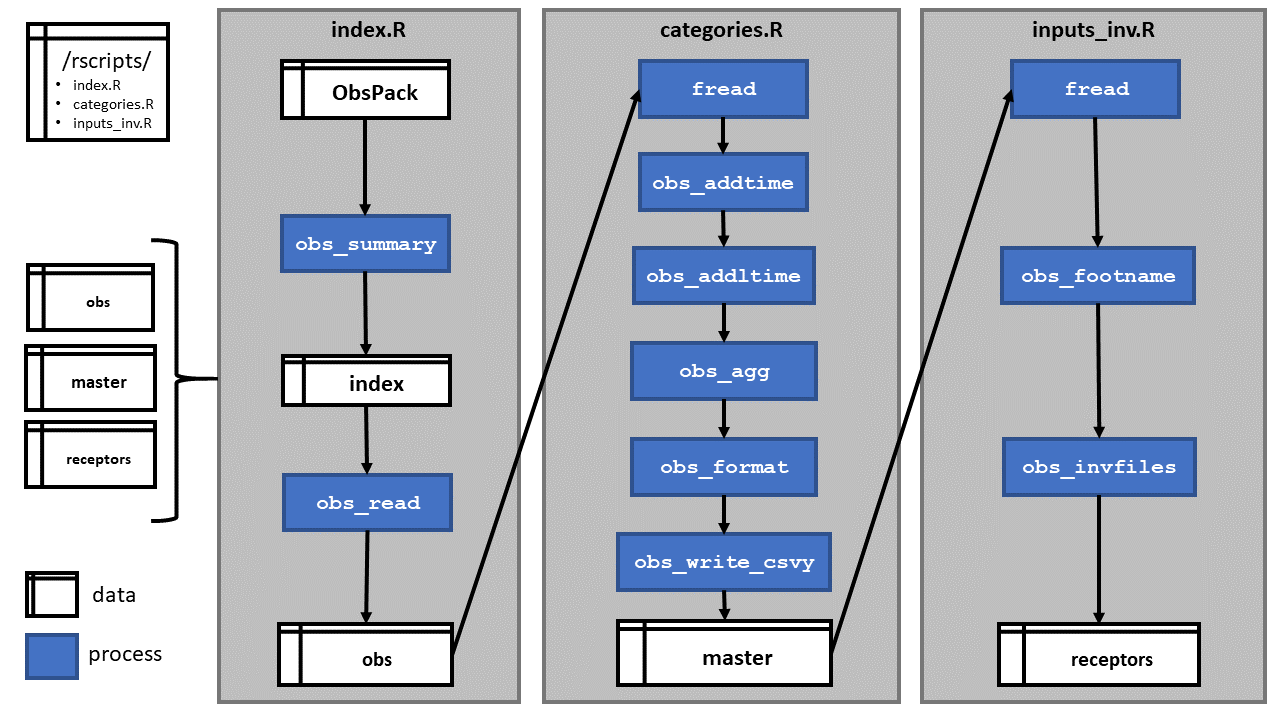
\includegraphics[width=1\linewidth,height=0.5\textheight]{flow/Slide1} \caption{Methane observations (ppb) by towers-insitu}\label{fig:flow}
\end{figure}

The file \texttt{index.R} creates a summary of ObsPack, generates the
directories master, receptor and obs, and store the summaries in obs
directory for each category. Then, the scripts for each category are run
to generate the master and receptor files. The next step consists in
running HYSPLIT and obtaining footprints (not in the scope of this
manuscript). At last, the script \texttt{inputs\_inv.R} checks each
footprint file for each category and generates the final receptor list
files. The process is described in detail in the following example for
tower insitu.

The first step consists in constructing a summary for the ObsPack. This
is required to read the data, but also, identify agl, which is present
in some of the file names. This function returns a data.frame.
Optionally, the user can indicate a path to store the data.frame.
obs\_summary also prints a summary of the data. The second argument is
the categories, and by default includes the categories shown below, to
account for all the files. Then the summary data.frame contains the
columns id as the full path to each file, name which is the name or
relative path of the file, n which is just an id, sector such as tower,
and the column agl which indicates the agl indicated in the name of the
file if available. To read the documentation of this function, the user
must run \texttt{?obs\_summary}.

\begin{Shaded}
\begin{Highlighting}[]
\NormalTok{categories }\OtherTok{\textless{}{-}} \FunctionTok{c}\NormalTok{(}\StringTok{"aircraft{-}pfp"}\NormalTok{,}\StringTok{"aircraft{-}insitu"}\NormalTok{,}\StringTok{"surface{-}insitu"}\NormalTok{,}
  \StringTok{"aircore"}\NormalTok{,}\StringTok{"surface{-}pfp"}\NormalTok{,}\StringTok{"tower{-}insitu"}\NormalTok{,}\StringTok{"shipboard{-}insitu"}\NormalTok{,}\StringTok{"flask"}\NormalTok{)}
\NormalTok{obs }\OtherTok{\textless{}{-}} \StringTok{"../../../obspack\_ch4\_1\_GLOBALVIEWplus\_v4.0\_2021{-}10{-}14/data/txt"}
\NormalTok{index }\OtherTok{\textless{}{-}} \FunctionTok{obs\_summary}\NormalTok{(}\AttributeTok{obs =}\NormalTok{ obs, }\AttributeTok{verbose =}\NormalTok{ F)}
\end{Highlighting}
\end{Shaded}

\begin{table}

\caption{\label{tab:kable}Summary of ObsPack}
\centering
\begin{tabular}[t]{l|r}
\hline
sector & N\\
\hline
aircraft-pfp & 40\\
\hline
aircraft-insitu & 11\\
\hline
flask & 101\\
\hline
surface-insitu & 124\\
\hline
aircore & 1\\
\hline
surface-pfp & 33\\
\hline
tower-insitu & 51\\
\hline
shipboard-insitu & 1\\
\hline
Total sectors & 362\\
\hline
\end{tabular}
\end{table}

There are 362 files in the ObsPack directory. The printed information
also shows the total at the bottom, as the sum of the individual file by
sector. This is to ensure that the sum of files is equal to the total
number of files found, shown at the top. furthermore, the printed
information also shows that there are 136 files with the agl explicitly
mentioned in the name of the file. Sometimes we need more information
about the site. For instance, what do the observations start and end.
Then, we added the function \texttt{obs\_table}, which calculates
statistics summary of ``time'' and other numeric variables by file name,
sector, site, altitude and mode. For instance, the observations in the
site ``SCT'' in South Carolina, USA, were between ``2015-08-19 21:30:00
UTC'' and ``2020-12-31 23:30:00 UTC''. In figure @ref(fig:tiobs) we see
the average of methane concentrations over each tower-insitu site.
Higher concentration are found over Russia. Over the United States
(U.S.), most of towers are found in the south to east coast.

\begin{figure}
\centering
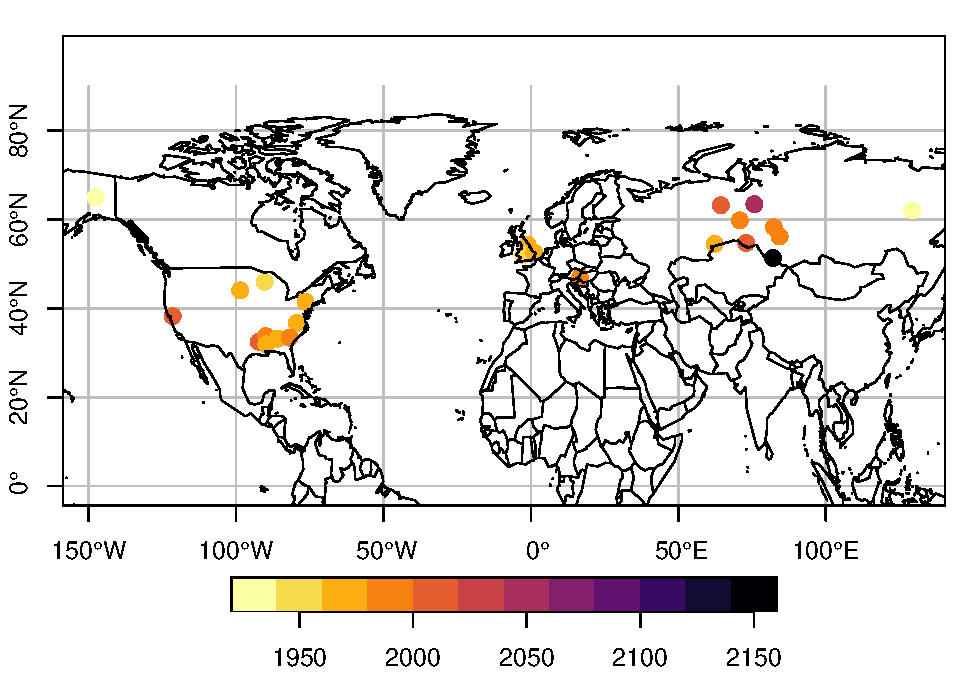
\includegraphics{paper_elsevier_files/figure-latex/tiobs-1.pdf}
\caption{Methane observations (ppb) by towers-insitu}
\end{figure}

\hypertarget{functions}{%
\subsection{Functions}\label{functions}}

The \texttt{robspack} functions are shown in table 1.

Table 1. Functions and classes in \texttt{robspack}.

\begin{longtable}[]{@{}
  >{\raggedright\arraybackslash}p{(\columnwidth - 2\tabcolsep) * \real{0.3108}}
  >{\raggedright\arraybackslash}p{(\columnwidth - 2\tabcolsep) * \real{0.6892}}@{}}
\toprule\noalign{}
\begin{minipage}[b]{\linewidth}\raggedright
Function
\end{minipage} & \begin{minipage}[b]{\linewidth}\raggedright
Description
\end{minipage} \\
\midrule\noalign{}
\endhead
\bottomrule\noalign{}
\endlastfoot
\texttt{invfile} & Class with \texttt{print}, \texttt{summary} and
\texttt{plot} methods \\
\texttt{obs\_addltime()} & Add local time based on metadata and
longitude \\
\texttt{obs\_addtime()} & Add UTC time \\
\texttt{obs\_agg()} & Aggregates ObsPack by time \\
\texttt{obs\_find\_receptors()} & Find expected receptors and NetCDF
files \\
\texttt{obs\_format()} & Format for some columns of data.table \\
\texttt{obs\_freq()} & Return numeric vector in intervals \\
\texttt{obs\_invfiles()} & Construct \texttt{invfile} objects \\
\texttt{obs\_list.dt()} & Rbind list of data.frames with different
names \\
\texttt{obs\_meta()} & Reads ObsPack metadata \\
\texttt{obs\_out()} & Outersect, opposed as intersect \\
\texttt{obs\_rbind()} & Rbind data.frames with different names \\
\texttt{obs\_read()} & Read files, and add metadata as columns \\
\texttt{obs\_read\_csvy()} & Read csvy file and prints yaml header \\
\texttt{obs\_roundtime()} & Round seconds from ``POSIXct'' ``POSIXt''
classes \\
\texttt{obs\_summary()} & Construct summary of ObsPack as a
data.frame \\
\texttt{obs\_table()} & Return a data.frame with summary of data \\
\texttt{obs\_trunc()} & Trunc numbers with a desired number of
decimals \\
\texttt{obs\_write()} & Write CSVY to disk, YAML followed by
tabulated \\
\end{longtable}

\hypertarget{application-for-towers-in-situobspack-summary}{%
\section{Application for towers in situObsPack
summary}\label{application-for-towers-in-situobspack-summary}}

\hypertarget{read-data}{%
\subsection{Read data}\label{read-data}}

Once the summary is built, the function obs\_read will read the files
available in the index file previously generated. Here we selected the
category ``tower-insitu''. The argument verbose prints which files are
being read each time, by default. At the end, this function prints the
total number of observations by type of altitude (agl or asl).

\begin{Shaded}
\begin{Highlighting}[]
\NormalTok{df }\OtherTok{\textless{}{-}} \FunctionTok{obs\_read}\NormalTok{(}\AttributeTok{index =}\NormalTok{ index,}
               \AttributeTok{categories =} \StringTok{"tower{-}insitu"}\NormalTok{,}
               \AttributeTok{verbose =} \ConstantTok{FALSE}\NormalTok{)}
\end{Highlighting}
\end{Shaded}

We added a function to plot the data read from ObsPack. The y-axis is
the field value and the x-axis is by default time. The data illustrated
sorted by color is the field site\_code, with the default number of 3
sites. The argument pal is to define the color palette, used by the
internally imported function cptcity::cpt.

\begin{Shaded}
\begin{Highlighting}[]
\FunctionTok{obs\_plot}\NormalTok{(}\AttributeTok{dt =}\NormalTok{ df, }\AttributeTok{time =} \StringTok{"time"}\NormalTok{, }\AttributeTok{yfactor =} \FloatTok{1e+09}\NormalTok{, }\AttributeTok{cex =} \FloatTok{0.5}\NormalTok{)}
\end{Highlighting}
\end{Shaded}

\begin{verbatim}
## Found the following sites: 
##  [1] AZV   BRZ   BSD   CRV   DEM   DVV   GCI01 GCI02 GCI03 GCI04 HUN   IGR  
## [13] KRS   LEF   MRC   NOY   RGL   SCT   SVV   TAC   VGN   WGC   WSD   YAK  
## Plotting the following sites: 
## [1] AZV BRZ
\end{verbatim}

\begin{figure}
\centering
\includegraphics{paper_elsevier_files/figure-latex/obsplot-1.pdf}
\caption{First two sites in ObsPack}
\end{figure}

Before sub setting the data, tower-insitu has about 2.32 million
observations. These observations are made between 2004 and 2020. The
identification of the altitude and type is critical, then we developed
an approach based on the availability of data:

\begin{enumerate}
\def\labelenumi{\arabic{enumi}.}
\tightlist
\item
  Identify agl from the name of the tile.
\item
  If agl not present, search fill\_values used in elevation and
  transform them into NA (not available)
\item
  If agl is not present, agl = altitude - elevation.
\item
  If there are some NA in elevation, will result some NA in agl
\item
  A new column is added named altitude\_final to store agl or asl
\item
  Another column named type\_altitude is added to identify agl or asl.
\item
  If there is any case NA in altitude\_final, type\_altitude is ``not
  available''
\end{enumerate}

\hypertarget{filtering}{%
\subsection{Filtering}\label{filtering}}

ObsPack includes global observations and sometimes we need to extract
data for a specific region and periods of time. In this part we include
spatial and temporal parameters to filter data. The year of interest is
2020, but we also included December of 2019 and January of 2021. The
spatial filtering is done by using the coordinates, in this case
covering North America. After filtering by space and time, we have
\ensuremath{2.322369\times 10^{6}} million observations.

\begin{Shaded}
\begin{Highlighting}[]
\NormalTok{north }\OtherTok{\textless{}{-}} \DecValTok{80}
\NormalTok{south }\OtherTok{\textless{}{-}} \DecValTok{10}
\NormalTok{west }\OtherTok{\textless{}{-}} \SpecialCharTok{{-}}\DecValTok{170}
\NormalTok{east }\OtherTok{\textless{}{-}} \SpecialCharTok{{-}}\DecValTok{50}
\NormalTok{max\_altitude }\OtherTok{\textless{}{-}} \DecValTok{8000}
\NormalTok{evening }\OtherTok{\textless{}{-}} \DecValTok{14}\SpecialCharTok{:}\DecValTok{15}

\NormalTok{yy }\OtherTok{\textless{}{-}} \DecValTok{2020}
\NormalTok{df }\OtherTok{\textless{}{-}} \FunctionTok{rbind}\NormalTok{(df[year }\SpecialCharTok{==}\NormalTok{ yy }\SpecialCharTok{{-}} \DecValTok{1} \SpecialCharTok{\&}\NormalTok{ month }\SpecialCharTok{==} \DecValTok{12}\NormalTok{],}
\NormalTok{            df[year }\SpecialCharTok{==}\NormalTok{ yy],}
\NormalTok{            df[year }\SpecialCharTok{==}\NormalTok{ yy }\SpecialCharTok{+} \DecValTok{1} \SpecialCharTok{\&}\NormalTok{ month }\SpecialCharTok{==} \DecValTok{1}\NormalTok{])}

\NormalTok{df }\OtherTok{\textless{}{-}}\NormalTok{ df[altitude\_final }\SpecialCharTok{\textless{}}\NormalTok{ max\_altitude }\SpecialCharTok{\&}
\NormalTok{           latitude }\SpecialCharTok{\textless{}}\NormalTok{ north }\SpecialCharTok{\&}
\NormalTok{           latitude }\SpecialCharTok{\textgreater{}}\NormalTok{ south }\SpecialCharTok{\&}
\NormalTok{           longitude }\SpecialCharTok{\textless{}}\NormalTok{ east }\SpecialCharTok{\&}
\NormalTok{           longitude }\SpecialCharTok{\textgreater{}}\NormalTok{ west]}
\end{Highlighting}
\end{Shaded}

\hypertarget{time}{%
\subsection{Time}\label{time}}

The function obs\_addtime adds time columns timeUTC, timeUTC\_start
which shows the start time of each observation and timeUTC\_end which
shows the end time for each observation. Then we need to identify the
local time with the function add\_ltime. This is important because to
identify observations in the evening in local time for modeling
purposes. add\_ltime uses two methods, first identifying the time
difference with utc by identifying the metadata column
``site\_utc2lst''. If this information is not available, with the
aircrafts for instance, the local time is calculated with an
approximation based on longitude:

\[
lt = UTC + longitude/15 * 60 * 60
\] Where lt is the local time, UTC the time, and longitude is the
coordinate. Then, the time is cut every two hours. We also identify the
local time to select evening hours.

\begin{Shaded}
\begin{Highlighting}[]
\NormalTok{df2 }\OtherTok{\textless{}{-}} \FunctionTok{obs\_addtime}\NormalTok{(df)}
\end{Highlighting}
\end{Shaded}

\begin{verbatim}
## Adding timeUTC
## Adding timeUTC_start
## Adding timeUTC_end
\end{verbatim}

\begin{Shaded}
\begin{Highlighting}[]
\NormalTok{df2}\SpecialCharTok{$}\NormalTok{timeUTC }\OtherTok{\textless{}{-}} \FunctionTok{cut}\NormalTok{(}\AttributeTok{x =}\NormalTok{ df2}\SpecialCharTok{$}\NormalTok{timeUTC}\SpecialCharTok{+}\DecValTok{3600}\NormalTok{,}
                   \AttributeTok{breaks =} \StringTok{"2 hour"}\NormalTok{) }\SpecialCharTok{|\textgreater{}}
  \FunctionTok{as.character}\NormalTok{() }\SpecialCharTok{|\textgreater{}}
  \FunctionTok{as.POSIXct}\NormalTok{(}\AttributeTok{tz =} \StringTok{"UTC"}\NormalTok{)}
\NormalTok{df3 }\OtherTok{\textless{}{-}} \FunctionTok{obs\_addltime}\NormalTok{(df2)}
\NormalTok{df3 }\OtherTok{\textless{}{-}}\NormalTok{ df3[lh }\SpecialCharTok{\%in\%}\NormalTok{ evening]}
\end{Highlighting}
\end{Shaded}

Now there are 8391 observations. At this point we can calculate the
averages of several columns by the cut time. The function obs\_agg does
this aggregation as shown in the following lines of code. The argument
gby establish the function used to aggregate cols, in this case the
function ``mean'' by time and altitude. Finally, we add local time
again.

\begin{Shaded}
\begin{Highlighting}[]
\NormalTok{df4 }\OtherTok{\textless{}{-}} \FunctionTok{obs\_agg}\NormalTok{(}\AttributeTok{dt =}\NormalTok{ df3,}
               \AttributeTok{gby =} \StringTok{"mean"}\NormalTok{,}
               \AttributeTok{cols =} \FunctionTok{c}\NormalTok{(}\StringTok{"value"}\NormalTok{, }\StringTok{"latitude"}\NormalTok{, }\StringTok{"longitude"}\NormalTok{, }\StringTok{"type\_altitude"}\NormalTok{,}
                        \StringTok{"dif\_time"}\NormalTok{, }\StringTok{"year\_end"}\NormalTok{, }\StringTok{"site\_utc2lst"}\NormalTok{),}
               \AttributeTok{verbose =} \ConstantTok{FALSE}\NormalTok{,}
               \AttributeTok{byalt =} \ConstantTok{TRUE}\NormalTok{)}
\end{Highlighting}
\end{Shaded}

\begin{verbatim}
## Detecting dif_time. Adding ending times
\end{verbatim}

\begin{Shaded}
\begin{Highlighting}[]
\NormalTok{df5 }\OtherTok{\textless{}{-}} \FunctionTok{obs\_addltime}\NormalTok{(df4)}
\end{Highlighting}
\end{Shaded}

Now there are 4394 observations. Towers can have observations at
different heights. Here we need to select one site with the observations
registered at the highest height. The column with the height is named
altitude\_final and the max altitude was named max\_altitude. Then, we
print the altitudes of each site.

\begin{Shaded}
\begin{Highlighting}[]
\NormalTok{df5[,}
\NormalTok{    max\_altitude }\SpecialCharTok{:=} \FunctionTok{max}\NormalTok{(altitude\_final),}
\NormalTok{    by }\OtherTok{=}\NormalTok{ site\_code]}
\NormalTok{df5[,}
    \FunctionTok{c}\NormalTok{(}\StringTok{"site\_code"}\NormalTok{,}
      \StringTok{"altitude\_final"}\NormalTok{,}
      \StringTok{"max\_altitude"}\NormalTok{)] }\SpecialCharTok{|\textgreater{}} \FunctionTok{unique}\NormalTok{()}
\end{Highlighting}
\end{Shaded}

\begin{verbatim}
##     site_code altitude_final max_altitude
##  1:       CRV           17.0           32
##  2:       CRV           32.0           32
##  3:       CRV            4.9           32
##  4:       LEF          122.0          396
##  5:       LEF           30.0          396
##  6:       LEF          396.0          396
##  7:       SCT          305.0          305
##  8:       SCT           31.0          305
##  9:       SCT           61.0          305
## 10:       WGC           30.0          483
## 11:       WGC          483.0          483
## 12:       WGC           91.0          483
\end{verbatim}

\hypertarget{saving-master-as-text-and-csvy}{%
\subsection{Saving master as text and
csvy}\label{saving-master-as-text-and-csvy}}

Now that we have all the required information, we can save the files.
Here, we name the data.frame as master, because it contains all the
information. This is important because some fields can be used in the
future, and for traceability. For convenience, time variables are
transformed into character before writing into the disk. The separation
is space '' ``.

\begin{Shaded}
\begin{Highlighting}[]
\NormalTok{master }\OtherTok{\textless{}{-}}\NormalTok{ df5}
\NormalTok{master}\SpecialCharTok{$}\NormalTok{timeUTC }\OtherTok{\textless{}{-}} \FunctionTok{as.character}\NormalTok{(master}\SpecialCharTok{$}\NormalTok{timeUTC)}
\NormalTok{master}\SpecialCharTok{$}\NormalTok{timeUTC\_end }\OtherTok{\textless{}{-}} \FunctionTok{as.character}\NormalTok{(master}\SpecialCharTok{$}\NormalTok{timeUTC\_end)}
\NormalTok{master}\SpecialCharTok{$}\NormalTok{local\_time }\OtherTok{\textless{}{-}} \FunctionTok{as.character}\NormalTok{(master}\SpecialCharTok{$}\NormalTok{local\_time)}

\FunctionTok{fwrite}\NormalTok{(master, }
       \AttributeTok{file =} \StringTok{"tower\_insitu\_2020.txt"}\NormalTok{,}
       \AttributeTok{sep =} \StringTok{" "}\NormalTok{)}
\end{Highlighting}
\end{Shaded}

The format Comma Separated Value with YAML (CSVY)\footnote{https://csvy.org/}
consists in a typical CSV with a YAML header. The function obs\_write
includes the argument notes which allows adding custom notes at the
header of the file. Below the notes, obs\_write adds the output of the R
function \texttt{str}, which provides a vertical summary of the data,
known as structure.

\begin{Shaded}
\begin{Highlighting}[]
\FunctionTok{obs\_write\_csvy}\NormalTok{(}\AttributeTok{dt =}\NormalTok{ master,}
              \AttributeTok{notes =} \StringTok{"tower 2020"}\NormalTok{,}
              \AttributeTok{out =} \StringTok{"tower\_insitu\_2020.csvy"}\NormalTok{)}
\end{Highlighting}
\end{Shaded}

To check the YAML header we read the first 38 lines of the files that
were generated. Here we can see the column names, type of data and first
observations. The YAML header is delimited by the characters ``- - -''
(not shown here).

\begin{Shaded}
\begin{Highlighting}[]
\FunctionTok{readLines}\NormalTok{(}\StringTok{"tower\_insitu\_2020.csvy"}\NormalTok{)[}\DecValTok{1}\SpecialCharTok{:}\DecValTok{38}\NormalTok{]}
\end{Highlighting}
\end{Shaded}

\hypertarget{saving-receptors}{%
\subsection{Saving receptors}\label{saving-receptors}}

We need to filter some columns from the master files in a new object
called receptors. This is needed because internally we run HYSPLIT
\citep{hy} using the information from the receptors. In the case of a
tower, we need to select observations with the highest altitude. The
specific columns are selected as shown on the following code. We are
selecting the ending times, because later HYSPLIT is run backwards based
on the time of measurement, between ending and starting times. The
columns about time are formatted to have two characters. For instance,
the month 1, is formatted as ``01''. We also need to filter for
type\_altitude equal 0, representing agl observations , or equal to 1,
asl.

\begin{Shaded}
\begin{Highlighting}[]
\NormalTok{receptor }\OtherTok{\textless{}{-}}\NormalTok{ master[altitude\_final }\SpecialCharTok{==}\NormalTok{ max\_altitude,}
                   \FunctionTok{c}\NormalTok{(}\StringTok{"site\_code"}\NormalTok{,}
                     \StringTok{"year"}\NormalTok{, }\StringTok{"month"}\NormalTok{, }\StringTok{"day"}\NormalTok{,}
                     \StringTok{"hour"}\NormalTok{, }\StringTok{"minute"}\NormalTok{, }\StringTok{"second"}\NormalTok{,}
                     \StringTok{"latitude"}\NormalTok{, }\StringTok{"longitude"}\NormalTok{,}
                     \StringTok{"altitude\_final"}\NormalTok{, }\StringTok{"type\_altitude"}\NormalTok{,}
                     \StringTok{"year\_end"}\NormalTok{, }\StringTok{"month\_end"}\NormalTok{, }\StringTok{"day\_end"}\NormalTok{, }\StringTok{"hour\_end"}\NormalTok{,}
                     \StringTok{"minute\_end"}\NormalTok{, }\StringTok{"second\_end"}\NormalTok{)]}
\NormalTok{receptor}\SpecialCharTok{$}\NormalTok{altitude\_final }\OtherTok{\textless{}{-}} \FunctionTok{round}\NormalTok{(receptor}\SpecialCharTok{$}\NormalTok{altitude\_final)}
\NormalTok{receptor }\OtherTok{\textless{}{-}} \FunctionTok{obs\_format}\NormalTok{(receptor)}

\ControlFlowTok{if}\NormalTok{(}\FunctionTok{nrow}\NormalTok{(receptor\_agl) }\SpecialCharTok{\textgreater{}} \DecValTok{0}\NormalTok{) \{}
  \FunctionTok{fwrite}\NormalTok{(}\AttributeTok{x =}\NormalTok{ receptor\_agl,}
         \AttributeTok{file =} \StringTok{"paper/receptor\_tower\_insitu\_2020\_AGL.txt"}\NormalTok{),}
\NormalTok{  sep }\OtherTok{=} \StringTok{" "}\ErrorTok{)}\NormalTok{\}}

\ControlFlowTok{if}\NormalTok{(}\FunctionTok{nrow}\NormalTok{(receptor\_asl) }\SpecialCharTok{\textgreater{}} \DecValTok{0}\NormalTok{) \{}
  \FunctionTok{fwrite}\NormalTok{(}\AttributeTok{x =}\NormalTok{ receptor\_asl,}
         \AttributeTok{file =} \StringTok{"paper/receptor\_tower\_insitu\_2020\_ASL.txt"}\NormalTok{),}
\NormalTok{  sep }\OtherTok{=} \StringTok{" "}\ErrorTok{)}\NormalTok{\}}
\end{Highlighting}
\end{Shaded}

\hypertarget{recommendation-for-other-applications}{%
\subsection{Recommendation for other
applications}\label{recommendation-for-other-applications}}

The approach to generate receptors depends on each type of observation
and other considerations. For instance, aircraft with continuous
observations at each second can be filtered and averaged every 20
seconds. In that way, the footprints are still representative and it
would not be necessary to run HYSPLIT every second. Of course, it
depends on the application and objective of the study. For this
manuscript, we are presenting the generation of receptors based on tower
observations.

\hypertarget{conclusion}{%
\section{Conclusion}\label{conclusion}}

In this manuscript we presented an robskpack, an R package to read and
process CH4 ObsPack GLOBALVIEW+ published by the Global Monitoring
Laboratory (GML) from the National Oceanographic and Atmospheric
Administration (NOAA). robspack reads the text data which have different
headers and organizes them in a common format. Then, this software
applies calculations to filter observations by time and space. Finally,
this software generates receptors in a suitable format that allows it to
run HYSPLIT and generate footprints. This software does not provide
methods to run HYSPLIT, but the user can follow the site
https://www.ready.noaa.gov/HYSPLIT.php.

\hypertarget{acknowledgements}{%
\section{Acknowledgements}\label{acknowledgements}}

Funding: This project is funded by the NOAA Climate Program Office AC4
and COM programs (NA21OAR4310233 / NA21OAR4310234). This research was
supported by the NOAA cooperative agreement NA22OAR4320151.

\renewcommand\refname{References}
\bibliography{mybibfile.bib}


\end{document}
